% \documentclass[conference]{IEEEtran}
\documentclass[onecolumn, 12pt]{IEEEtran}
% \documentclass[12pt]
\IEEEoverridecommandlockouts
% The preceding line is only needed to identify funding in the first footnote. If that is unneeded, please comment it out.
\usepackage{setspace}
\doublespacing
\usepackage{cite}
\usepackage{wrapfig}
\usepackage{algorithm}
\usepackage{algorithmic}
\usepackage{amsmath,amssymb,amsfonts}
\usepackage{graphicx}
\usepackage{caption}
\usepackage{textcomp}
\usepackage{multirow}
\usepackage{indentfirst}
% \usepackage[numbers,sort&compress]{natbib}
\setlength{\parindent}{1em}
\usepackage{hyperref}
\hypersetup{
    colorlinks=true,
    linkcolor=black,
    filecolor=black,
    urlcolor=black
}
\usepackage{color}
\newcommand{\add}[1]{\textcolor{blue}{#1}}
\newcommand{\delete}[1]{\textcolor{red}{#1}}
\definecolor{darkgrn}{rgb}{0, 0.8, 0}
\newcommand{\modified}[1]{\textcolor{darkgrn}{#1}}
\usepackage{gensymb}
%%

\def\BibTeX{{\rm B\kern-.05em{\sc i\kern-.025em b}\kern-.08em
    T\kern-.1667em\lower.7ex\hbox{E}\kern-.125emX}}
\begin{document}

\title{Proposal Topic \\
BitCoin Exchange Trust Network Analysis
}

\author{\IEEEauthorblockN{Shiv Raj Pant, Xiaoqin Fu}\\
\IEEEauthorblockA{School of Electrical Engineering and Computer Science\\
Washington State University\\
Pullman, WA\\
Email: \{shiv.pant,  xiaoqin.fu\}@wsu.edu}}

\maketitle
\section{Introduction}
BitCoin was developed in 2008 and 2009 as a radical new concept for money and currency~\cite{nakamoto2008bitcoin} using blockchain technology.
Blockchain is a distributed database which keeps record in a distributed fashion.
Figure~\ref{fig:blkchain} shows the schematic diagram of blockchain.
A block encrypts the data using cryptographic hash function, such as SHA-256, and keeps record of next available block for traversing the blocks.
Records are stored in a tree structure where the leaves stores the transaction information and other intermediate nodes store the hash values. The root of this tree belongs in a block containing the hash value generated from child nodes.
The timestamp in a block is used to synchronize the position of a block in blockchain.
A block also contains NONCE value, which is random unique number for a specific block.
\begin{figure}[htbp]
\centerline{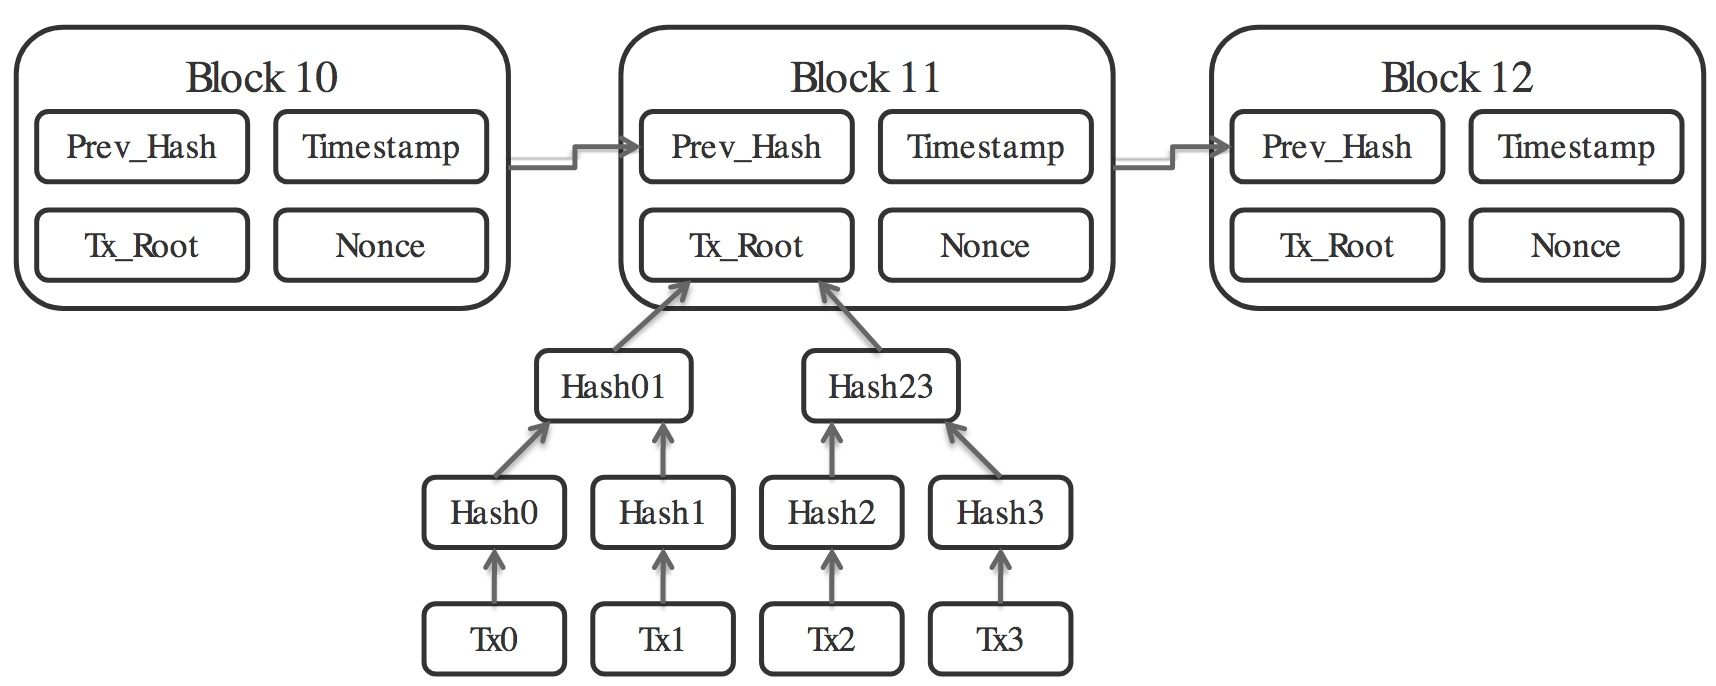
\includegraphics[width=\columnwidth]{blockchain.jpeg}}
\caption{Blocks are connected in a chained fashion where each block contains
many transaction records. This figure regenerated from~\cite{blkchaindiag}.}

\label{fig:blkchain}
\end{figure}

Our research focuses on study data from a BITCOIN marketplace with interactions and ratings~\cite{aw2018analyzing}.
They are (directed) weighted signed network (WSN) in which edge corresponds to some weight, the rating from user u to user v~\cite{moindrot2017trust}.
They forms webs of trust between users allowing two unknown users to perform a transaction based on the aggregated trust~\cite{moindrot2017trust}.

\section{Methodology}
Our paper is to study the two trust networks: Bitcoin OTC web of trust network and Bitcoin Alpha web of trust network, and analyze the relationship between price and trust. Moveover, we will predict edge weights from time stamp data in the data sets.
For the experiment, we will extract both topological and non-topological features from the networks~\cite{liben2007link}~\cite{al2006link}~\cite{davis2011multi}.
\section{Data}
We will use two data sets, soc-sign-bitcoin-otc and soc-sign-bitcoin-alpha, from~\cite{snapnets}.
OTC and Alpha are two Bitcoin exchanges, which are open market websites allowing users to buy and sell things~\cite{snapnets}.
The soc-sign-bitcoin-otc, Bitcoin OTC web of trust network, is a (directed) weighted signed network (WSN) with 5,881 nodes and 35,592 edges.
On Bitcoin OTC, people can build up trust to exchange bitcoins with ratings from -10 (total distrust) to 10 (total trust) which are associated with how much a user trusts another user~\cite{moindrot2017trust}. A high rating is mapping the high trust. The data set has the rating times recorded as seconds since Epoch~\cite{snapnets}.

And the soc-sign-bitcoin-alpha, Bitcoin Alpha web of trust network, is also a directed WSN with 3,783 nodes and 24,186 edges.
It is similar in almost every way to the soc-sign-bitcoin-otc. It also has ratings from -10 to 10 and the rating times. While the OTC network
is still active, the Alpha exchange is no longer active now~\cite{moindrot2017trust}.

\section{Related work}
\begin{itemize}
 \item
 \item
 \item
 \item
 \end{itemize}
\section{Tentative plan}
\begin{itemize}
 \item
 \item
 \item
 \item
\end{itemize}
\bibliographystyle{IEEEtran}
%\bibliographystyle{IEEEtran}

%\balance

\bibliography{References}

\end{document}
